\subsection{Загрузка файлов}
Для загрузки данных из формата INTEL HEX8M (.hex) необходимо выбрать его в меню "Open":

\begin{figure}[h!]
    \centering
    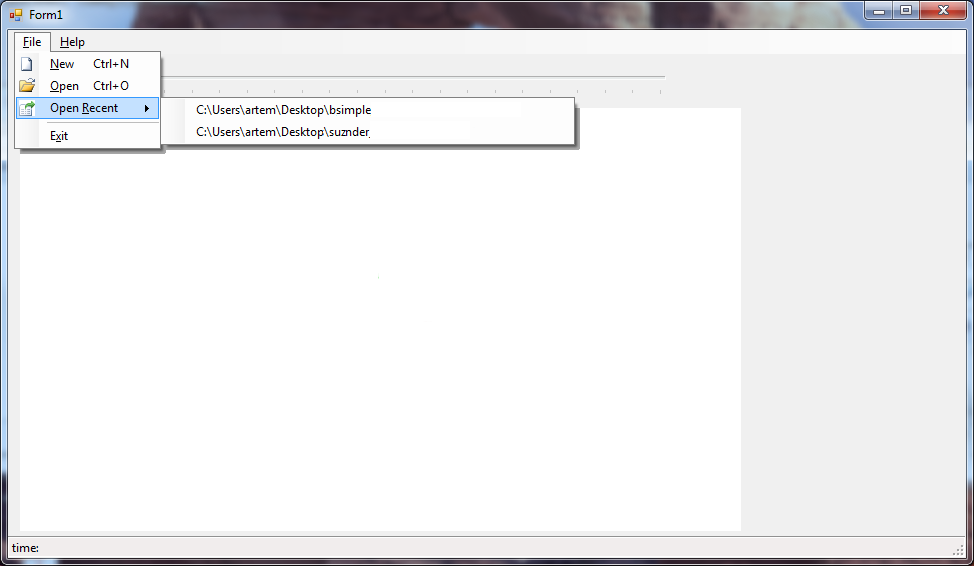
\includegraphics[width=0.8\textwidth]{../screenshots/file_menu_with_recent.png}
    \caption{Загрузка файла}
\end{figure}

Откроется диалог выбора файла:
\begin{figure}[h!]
    \centering
    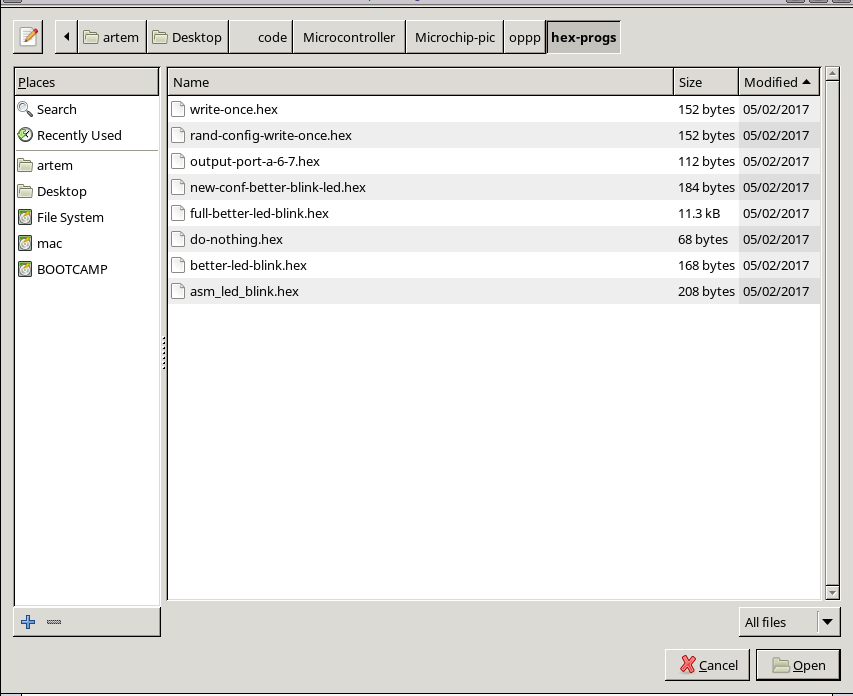
\includegraphics[width=0.5\textwidth]{../screenshots/open_file_dialog.png}
    \caption{Диалог выбора файла}
\end{figure}

После загрузки файла, его содержание будет отображенно в центральном окне.

\subsection{Изменение параметров программатора}
Есть панель для настоек работы программы позволяющая изменять следующие параметры:
\begin{my_enumerate}
\item Указать что требуется запись EEPROM памети без модификации програмной памяти микроконтроллера.
\item Указать что требуется проверить входной файл на ошибки.
\item Указать что требуется записать входной файл в програмную память и в EEPROM память микроконтроллера.
\item Поменять уровень колличества сообщений выводимих программой пользователю.
\item Отменить процесс программирования.
\end{my_enumerate}


\begin{figure}[h!]
    \centering
    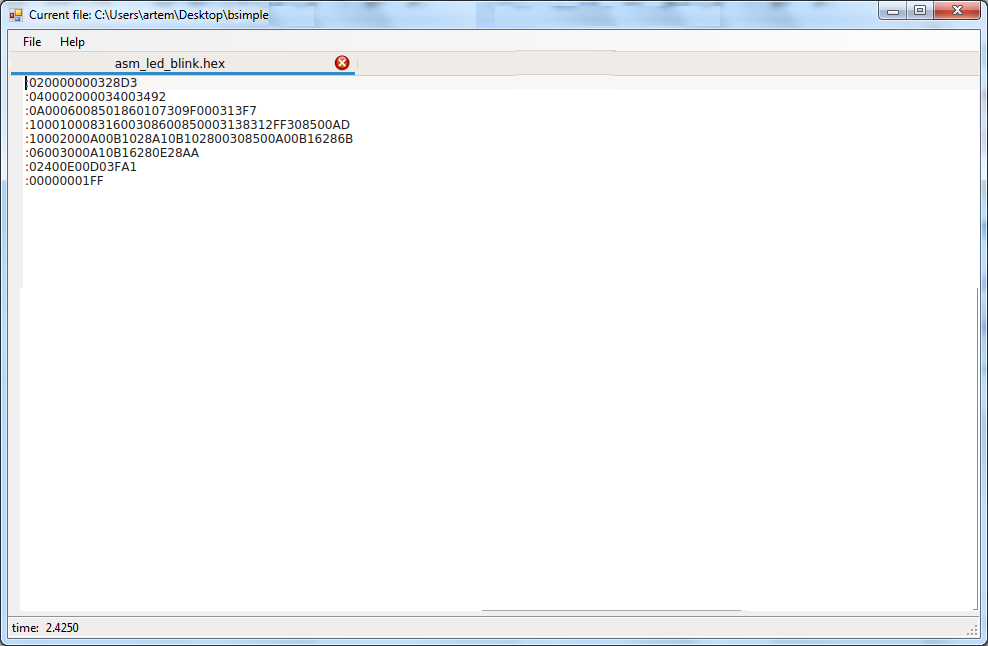
\includegraphics[width=0.8\textwidth]{../screenshots/interface_map.png}
    \caption{Настойки}
\end{figure}


\subsection{Всплывающие окна}
В случае если выбран файл не соответствующий требованиям входных данных отображается всплывающее окно:

\begin{figure}[h!]
    \centering
    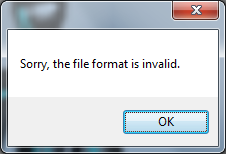
\includegraphics[width=0.3\textwidth]{../screenshots/error_message.png}
    \caption{Всплывающее окно}
\end{figure}


\subsection{Завершение работы с программой}
Происходит при нажатии на кнопку "Закрыть" в правом верхнем углу программы.
